% SUSY lectures for 1st year PhDs
\documentclass{beamer}
\usepackage{epstopdf}
\usetheme{iclpt}
\begin{document}

\title{Introduction to supersymmetry}
\subtitle{\textcolor{gray}{(and some supergravity)}}
\author{Sam Rogerson}
\institute{Imperial College London}
\date{\today}

\begin{frame}[plain]
  \titlepage
\end{frame}

\begin{frame}{Outline}
  \tableofcontents [part=1,hideallsubsections,]
  \tableofcontents [part=2,hideallsubsections,] 
  \tableofcontents [part=3,hideallsubsections,] 
  \tableofcontents [part=4,hideallsubsections,] 
  \tableofcontents [part=5,hideallsubsections,] 
  \tableofcontents [part=6,hideallsubsections,] 
\end{frame}


%%%%%%%%%%%%%%%%%%%%%%%%%%%%%%%%%%%%%%%%%%%%%%%%%%%%%%%%%%%%%%%%%%%%%%%%%%%%%%%
% Introduction
%---------------------------------
\part{What is supersymmetry}
\section{What is supersymmetry}
\frame{\partpage}
%---------------------------------

\subsection{Symmetries and Physics}
\begin{frame}{\insertsubsection}
  \begin{definition}
    If a system is invariant under an operation, the operation is said to represent a symmetry
    of the system.
  \end{definition}
  One can construct a Lagrangian (T-V) that embeds these symmetries and, using the
  Euler-Lagrange equations:
  \begin{equation*}
    \frac{\partial L}{q_{\alpha}}-\frac{d}{dt}\frac{\partial
    L}{\dot{q}_{\alpha}}=0,
  \end{equation*}
  derive the equations of motion for the system.
\end{frame}

\subsection{Charges and Conservation}
\begin{frame}{\insertsubsection}
  \begin{definition}{Noether's Theorem:}
    For each continuous symmetry of a system there is a corresponding conserved
    quantity
  \end{definition}
  \begin{itemize}
    \item Translational invariance: Linear Momentum
    \item Rotational invariance: Angular Momentum
    \item Time invariance: Energy
  \end{itemize}
  You can group these into a more compact notation:
  \begin{equation*}
    \textrm{Translations}\times \mathrm{SO}(3,1)
  \end{equation*}
  This is even more compactly known as the Poincar\'{e} group.
\end{frame}

\subsection{Symmetries in particle physics}
\begin{frame}{\insertsubsection}
  The Standard Model embeds three gauge\footnote{Invariant under some continuous
  group(s) of local transformations} symmetries:
  \begin{equation*}
    \mathrm{SU(3)_{C}\times SU(2)_{L}\times U(1)_{Y}}
  \end{equation*}
  These then predict various conservation laws:
  \begin{itemize}
    \item Colour charge ($C$)
    \item Weak Isospin ($T$)
    \item Weak hypercharge ($Y$)
    \item (Electric charge $Q = Y + T_{3}$)
  \end{itemize}
\end{frame}

\subsection{Additional Symmetry?}
\begin{frame}{\insertsubsection}
  Two distinct groups of particles:
  \begin{itemize}
    \item Bosons (spin $\in\mathbb{Z}$)
    \item Fermions (spin $\in(\mathbb{Z}\times\frac{1}{2})$)
  \end{itemize}
  In aiming for some unified theory we hope these would be indistinct.
  Posit the existence of symmetry that links fermions($f$) and bosons($b$)
  \begin{equation*}
    \hat{O}\left|f\right>=\left|b\right>;\hat{O}\left|b\right>=\left|f\right>;
  \end{equation*}
  And our conserved quantity is particle number, rather than lepton/baryon
  numbers individually.
\end{frame}

\subsection{Supersymmetry is...}
\begin{frame}{\insertsubsection}
  \begin{definition}{}
    A symmetry which relates the SM particles with spin \alert{S} to a second
    set of particles with spin \alert{S$\pm\frac{1}{2}$}.
  \end{definition}
  This means for every SM particle there is a corresponding `superpartner' with
  identical quantum numbers known as a \alert{sparticle}.
\end{frame}

%%%%%%%%%%%%%%%%%%%%%%%%%%%%%%%%%%%%%%%%%%%%%%%%%%%%%%%%%%%%%%%%%%%%%%%%%%%%%%%
% Why we need BSM
%---------------------------------
\section{Why we need BSM physics}
\part{Why we need BSM physics}
\frame{\partpage}
%---------------------------------
\subsection{Standard Model}
\begin{frame}{\insertsubsection}
  Plenty of evidence in favour of the Standard Model:
  \begin{itemize}
    \item Predictions: Existence of W boson,Z boson, charm quark, top quark and the gluon.
    \item Electroweak precision measurements: Mass and width of W and Z bosons.
  \end{itemize}
  It is, however, not complete
\end{frame}

\subsection{What it doesn't include}
\begin{frame}{\insertsubsection}
  \begin{itemize}
    \item Neutrino masses (Dirac/Majorana): can add terms, but not a direct result
    \item Gravity
    \item Dark Matter (`orthogonal' measurement)
  \end{itemize}
\end{frame}

\subsection{What does it get ``wrong''?}
\begin{frame}{\insertsubsection}
  \begin{itemize}
    \item Anomalous Magnetic Moment of the Muon: $(g-2)_{\mu}$
    \item Natural solution to W-scattering cross-section
    \item Higgs mass 
  \end{itemize}
  There is also the problem of naturalness:
  \begin{itemize}
    \item Why do we need 19 parameters to describe the SM?
    \item Why do we have a hierarchy problem? (Fine tuned cancellations to
    Fermi's constant)
  \end{itemize}
\end{frame}

\subsection{What is the hierarchy problem?}
\begin{frame}{\insertsubsection}
  \begin{itemize}
    \item Suppose SM valid up to GUT scale ($O(10^{15}\textrm{GeV})$) or even
    the Planck scale ($O(10^{19}\textrm{GeV})$)
    \item Weak interaction scale $\sim100\textrm{GeV}$
    \item If the inputs are chosen at these scales, the scalar mass terms in
    the Higgs sector must be chosen with an accuracy of $10^{-34}$ wrt the
    Planck mass.
  \end{itemize}
\end{frame}

\subsection{W-scattering cross-section}
\begin{frame}{\insertsubsection}
  One of the strongest indicators for something Higgs-like/BSM physics:
  \begin{itemize}
    \item Theory: the value explodes at some energy scale
    \item Violates perturbative unitarity
    \item Simplest solution: extra propagator = extra diagram $\rightarrow$
    cancels divergences
    \item This propagator is a scalar $\rightarrow$ Higgs
    \item Good evidence for upper limit on Higgs mass
  \end{itemize}
\end{frame}

\subsection{Divergent Higgs Mass}
\begin{frame}{\insertsubsection}
  \center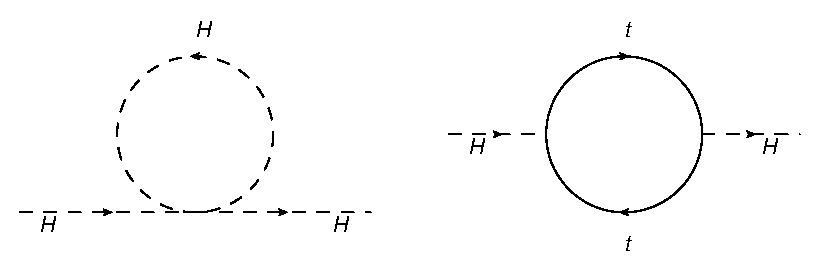
\includegraphics[scale=0.4]{oneloop.eps}\\
  The one loop scalar(left) and fermion(right) corrections to the Higgs mass.
  When calculated we find the following contributions:
  \begin{itemize}
    \item dirac fermion ($-\lambda_{f}\bar{f}f$):
    $\Delta m_{H}^{2}=-\frac{|\lambda_{f}|^2}{8\pi^{2}}\alert{\Lambda_{UV}^{2}}
    +\hdots$ 
    \item $\mathbb{C}$-scalar($-\lambda_{S}|H|^{2}|S|^{2}$): 
    $\Delta m_{H}^{2}= \frac{\lambda_{S}}{16\pi^{2}}\left[\Lambda_{UV}^{2}-2
    \alert{m_{S}^{2}}\ln\left(\Lambda_{UV}/m_{S}\right) \right]$
  \end{itemize}
  Here $\Lambda_{UV}$ is known as the `ultraviolet' cutoff - it regulates the loop
  integral, i.e $M=\int_{0}^{\Lambda_{UV}}\hdots$
\end{frame}

\subsection{Divergent Higgs Mass Part 2}
\begin{frame}{\insertsubsection}
  These corrections imply two important things:
  \begin{enumerate}
    \item A quadratic dependence on $\Lambda_{UV}$
    \item A quadratic dependence on $m_{S}$
  \end{enumerate}
  This means it is both sensitive to the scale of `new-physics', as well as the
  masses of the heaviest particles.  Strangely enough the latter problem arises
  even if we have no direct coupling between the SM Higgs and the unknown
  ``$S$''.
  \vfill\hfill We'll come back to this...
\end{frame}

\subsection{Why it could be SUSY}
\begin{frame}{\insertsubsection}
  \textcolor{gray}{Phenomenologically}
  While we haven't developed the details, yet, the extended particle spectrum
  gives hints at what it \alert{could} provide,
  \begin{itemize}
    \item Corrections to $\Delta(g-2)_{\mu}$
    \item A candidate for dark matter.
    \item Cancellation terms for the Higgs mass
    \item A solution to the Hierarchy problem
  \end{itemize}
\end{frame}


%%%%%%%%%%%%%%%%%%%%%%%%%%%%%%%%%%%%%%%%%%%%%%%%%%%%%%%%%%%%%%%%%%%%%%%%%%%%%%%
% Constructing SUSY
%---------------------------------
\part{Constructing the details of SUSY}
\frame{\partpage}
\section{Constructing the details of SUSY}
%---------------------------------

\subsection{Multiplets}
\begin{frame}{\insertsubsection}
In the standard model we arrange particles into the \alert{irriducible
representations} of the
algebra called multiplets,
  \begin{equation*}
    \binom{e_L}{\nu_{e}},\binom{u_{L}}{d_{L}}
  \end{equation*}
A similar approach is taken for SUSY; we form \alert{supermultiplets}, simply an
arrangement which contains both fermion and boson partner states
\end{frame}

\subsection{Multiplets Continued}
\begin{frame}{\insertsubsection}
  If $\left|\Omega\right>$ and $\left|\Omega^{\prime}\right>$ are both members of
  the same supermultiplet, then they are linear combinations of each other (with
  the SUSY operator $\hat{O}$ and $\hat{O}^{\dagger}$).
  \\ When constructing these multiplets we must ensure:
  \begin{equation*}
    n_{B}=n_{F}
  \end{equation*}
  where $n_{B}$ and $n_{F}$ are the bosonic and fermionic degrees of freedom
  respectively (this can be shown).
\\
  \alert{The simplest arrangement: single weyl fermion (2 spin states, $n_{F}=2$) and
  then 2 real scalars ($n_{B}=1$ each)}
\end{frame}

\subsection{More Multiplets}
\begin{frame}{\insertsubsection}
\textcolor{gray}{Note:
$2\times\mathbb{R}\textrm{-scalar}\equiv1\times\mathbb{C}\textrm{-scalar}$}\\
  The next simplest arrangement is a spin-1 vector boson ($n_{B}=2$), with a
  massless Weyl fermion as its superpartner.
  \\
  These two arrangements have names:
  \begin{itemize}
    \item spin-$1/2$ Weyl Fermion + $\mathbb{C}$-scalar: \alert{Chiral
    supermultiplet}
    \item spin-1 Vector boson + massless Weyl fermion: \alert{Gauge
    supermultiplet}
  \end{itemize}
\end{frame}

  
\subsection{Breaking SUSY}
\begin{frame}{\insertsubsection}
  If SUSY were an exact symmetry of the Lagrangian, then we would have,
  \begin{equation*}
    M_{\textrm{SM}}=M_{\textrm{SUSY}}
  \end{equation*}
  for all particles. If this were true, SUSY would be evident in experiments
  already.  We therefore expect SUSY to be broken to some degree, i.e. the mass
  scale of the particles is not completely restricted.
\alert{There is a much better reason than this...}
\end{frame}

\subsection{What is a gauge anomaly}
\begin{frame}{\insertsubsection}
  \begin{definition}
  A gauge anomaly is \alert{any} effect that breaks the gauge symmetry of the system, in our case the
  quantum field theory.
  \end{definition}
\end{frame}

\subsection{The Higgs Sector}
\begin{frame}{\insertsubsection}
  Naively one would expect the following:
  \begin{equation*}
    \textrm{Higgs } H \leftrightarrow \tilde{H}\textrm{ Higgsino} 
  \end{equation*}
  There is a \textcolor{gray}{(two)} problem\textcolor{gray}{(s)} with this,
  \begin{itemize}
    \item Introduction of a gauge anomaly, namely Higgsino ($S=\pm1/2$) has hypercharge
    $\textrm{Y}=\frac{1}{2}$, so we no longer have $\sum\textrm{Y}=0$ (our
    $U(1)$ gauge symmetry has been broken)
  \end{itemize}
\end{frame}

\subsection{The Higgs Sector Continued}
\begin{frame}{\insertsubsection}
  Can remedy this gauge anomaly by introducing a second higgs doublet, labelling
  the two (unsuggestively) $H_{u}$ and $H_{d}$.
  \begin{itemize}
    \item Opposite hypercharge (fixes the anomaly)
    \item $H_{u}$ now couples to up-type fermions ($u,c,t,\ell$)
    \item $H_{d}$ couples to down-type fermions ($d,s,b,\nu_{\ell}$)
  \end{itemize}
\end{frame}

\subsection{Supersymmetry is...}
\begin{frame}{\insertsubsection}
A symmetry that generates a second set of particles matching those in the SM
but with masses at a higher scale.
\begin{itemize}
  \item Each boson(fermion) has a corresponding (fermion)boson superpartner
  \item A second Higgs doublet is included, resulting in 5 physical Higgs bosons
\end{itemize}

\end{frame}

%%%%%%%%%%%%%%%%%%%%%%%%%%%%%%%%%%%%%%%%%%%%%%%%%%%%%%%%%%%%%%%%%%%%%%%%%%%%%%%
% Models of supersymmetry
%---------------------------------
\section{Models of supersymmetry}
\part{Models of supersymmetry}
\frame{\partpage}
%---------------------------------
\subsection{Minimal Supersymmetric Standard Model}
\begin{frame}{\insertsubsection}
  So far we have constructed what is known as the Minimal Supersymmetric
  Standard Model (MSSM)   
  \begin{itemize}
    \item super-partners for each SM particle
    \item softly-broken (mass differences, but no quadratic divergences)
  \end{itemize}
  This was motivated by the SM seeming ``unnatural'',
  \begin{itemize}
    \item  Number of parameters (19)
    \item  Energy scale ($M_{pl}$ vs. $M_{W}$)
  \end{itemize}
\end{frame}

\subsection{Not so natural...}
\begin{frame}{\insertsubsection}
  Unfortunately we have only really solved one of these problems,
  \begin{tabular}{l l }
    \checkmark & Energy scale \textcolor{gray}{almost}\\
    \ding{55} Parameters
  \end{tabular}
  To fully specify all the masses and couplings in the MSSM we need 108 free
  parameters.
  \\ \alert{Solution:} Choose some `natural` boundary condition to alleviate
  this problem.
\end{frame}

\subsection{CMSSM}
\begin{frame}{\insertsubsection}
  Running of the couplings:
  \includegraphics[height=5cm]{couple_sm.png}
\end{frame}

\subsection{NUHM1}
\begin{frame}{\insertsubsection}

\end{frame}

\subsection{mSUGRA}
\begin{frame}{\insertsubsection}
  Also called \alert{local supersymmetry}
\end{frame}


%%%%%%%%%%%%%%%%%%%%%%%%%%%%%%%%%%%%%%%%%%%%%%%%%%%%%%%%%%%%%%%%%%%%%%%%%%%%%%%
% How is this useful
%---------------------------------
\section{How is this useful?}
\part{How is this useful?}
\frame{\partpage}
%---------------------------------


\end{document}


